%-------------------------
% Resume in Latex
% Original author : Sourabh Bajaj
% Adaptation : Hyunggi Chang (changh95)
% License : MIT
%------------------------

\documentclass[letterpaper,11pt]{article}

\usepackage{latexsym}
\usepackage{kotex} % 한글 사용 가능! 
\usepackage[empty]{fullpage}
\usepackage{titlesec}
\usepackage{marvosym}
\usepackage[usenames,dvipsnames]{color}
\usepackage{verbatim}
\usepackage{enumitem}
\usepackage[hidelinks]{hyperref}
\usepackage{fancyhdr}
\usepackage[english]{babel}
\usepackage{tabularx}
\usepackage{booktabs}
\usepackage{amsmath}
\usepackage{tikz}
\usetikzlibrary{positioning, shapes.geometric, calc, backgrounds, arrows.meta}

\pagestyle{fancy}
\fancyhf{} % clear all header and footer fields
\fancyfoot{}
\renewcommand{\headrulewidth}{0pt}
\renewcommand{\footrulewidth}{0pt}

% Adjust margins
\addtolength{\oddsidemargin}{-0.5in}
\addtolength{\evensidemargin}{-0.5in}
\addtolength{\textwidth}{1in}
\addtolength{\topmargin}{-0.5in}
\addtolength{\textheight}{1.0in}

\urlstyle{same}

\raggedbottom
\raggedright
\setlength{\tabcolsep}{0in}

% Sections formatting
\titleformat{\section}{
  \vspace{-4pt}\scshape\raggedright\large
}{}{0em}{}[\color{black}\titlerule \vspace{-2pt}]

%-------------------------
% Custom commands - Do Look into this area, if you wish to customise further!
% 포맷이 마음에 들지 않으시다면 이 부분을 수정하세요!

\newcommand{\resumeItem}[1]{
  \item\small{
    {#1 \vspace{-2pt}}
  }
}

\newcommand{\resumeProject}[3]{
  \vspace{0pt}\item
    \begin{tabular*}{0.97\textwidth}[t]{l@{\extracolsep{\fill}}r}
      #1 & \small #2 \\
      {#3}
    \end{tabular*}\vspace{-5pt}
}

\newcommand{\resumeProjectNoDate}[2]{
  \vspace{0pt}\item
    #1 \\
    {#2}
    \vspace{-5pt}
}

\newcommand{\resumeSubProject}[2]{
  \item{
    {#1 \vspace{0pt}}
    {#2}
  }
}

\newcommand{\resumeSubheading}[4]{
  \vspace{-1pt}\item
    \begin{tabular*}{0.97\textwidth}[t]{l@{\extracolsep{\fill}}r}
      \textbf{#1} & \\
      \textit{\small#3} & \textit{\small #4} \\
    \end{tabular*}\vspace{-5pt}
}

\newcommand{\resumeSubItem}[2]{\resumeItem{#1}{#2}\vspace{-4pt}}

\renewcommand{\labelitemii}{$\circ$}

\newcommand{\resumeProjectListStart}{\begin{itemize}[leftmargin=*]}
\newcommand{\resumeProjectListEnd}{\end{itemize}}

\newcommand{\resumeSubProjectListStart}{\begin{itemize}[leftmargin=*]}
\newcommand{\resumeSubProjectListEnd}{\end{itemize}}

\newcommand{\resumeSubHeadingListStart}{\begin{itemize}[leftmargin=*]}
\newcommand{\resumeSubHeadingListEnd}{\end{itemize}}
\newcommand{\resumeItemListStart}{\begin{itemize}}
\newcommand{\resumeItemListEnd}{\end{itemize}\vspace{-5pt}}

%-------------------------------------------
%%%%%%  CV STARTS HERE  %%%%%%%%%%%%%%%%%%%%%%%%%%%%


\begin{document}

%----------HEADING-----------------
\begin{tabular*}{\textwidth}{l@{\extracolsep{\fill}}r}
  \textbf{\Large 경력 기술서} & Github: superhuman54 \\
  \href{https://superhuman54.github.io}{https://superhuman54.github.io} & Email : \href{mailto:YourEmail@gmail.com}{superhuman54.tech@gmail.com} \\
  {} & Mobile : (+82) 010-4691-0485
\end{tabular*}

%-----------PROJECTS-----------------
\section{\textbf{1. Spark History MCP + AI Agent로 Spark 분석 자동화}}
  \resumeProjectListStart
    \resumeProject
    {\textbf{소속}: 드림어스컴퍼니} {}
    
    \textbf{기여도}: 100\%
    
    {\textbf{상황}: 매일 110개 정도의 Spark 배치 작업을 운영하는 환경에서 작업 실패 시, 수동으로 Spark UI, CloudWatch Logs, EMR 콘솔을 오가며 수시간씩 디버깅해야 하는 비효율적인 운영 상황이 지속되고 있었습니다.
    
    \textbf{과제}: 
    \begin{enumerate}
        \item Spark 작업 실패 시 자동으로 원인을 분석하고 해결책을 제시하는 End-to-End 자동화 시스템을 구축
        \item 수동 디버깅 시간을 획기적으로 단축하고 운영 효율성을 향상
    \end{enumerate}

    \vspace{3mm}
    
    \resizebox{0.95\textwidth}{!}{ % 95% 너비로 자동 축소
    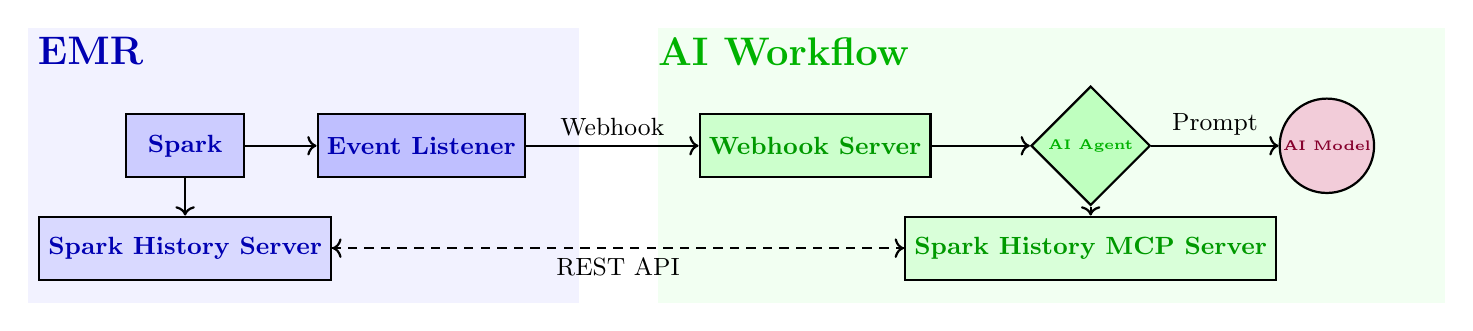
\begin{tikzpicture}[
        font=\sffamily,
        % 노드 스타일 정의
        client/.style={
            draw,
            circle,
            minimum size=0.1cm,
            thick,
            fill=blue!10,
            text=blue!70!black,
            font=\small\bfseries
        },
        spark/.style={
            draw,
            rectangle,
            minimum width=1.5cm,
            minimum height=0.8cm,
            thick,
            fill=blue!20,
            font=\small\bfseries,
            text=blue!70!black,
            align=center
        },
        historyServer/.style={
            draw,
            rectangle,
            minimum width=1.8cm,
            minimum height=0.8cm,
            thick,
            fill=blue!15,
            font=\small\bfseries,
            text=blue!70!black,
            align=center
        },
        eventListener/.style={
            draw,
            rectangle,
            minimum width=1.2cm,
            minimum height=0.8cm,
            thick,
            fill=blue!25,
            font=\small\bfseries,
            text=blue!70!black,
            align=center
        },
        webhookServer/.style={
            draw,
            rectangle,
            minimum width=1.5cm,
            minimum height=0.8cm,
            thick,
            fill=green!20,
            font=\small\bfseries,
            text=green!60!black,
            align=center
        },
        aiAgent/.style={
            draw,
            diamond,
            minimum width=0.3cm,
            minimum height=0.3cm,
            inner sep=2pt,
            thick,
            fill=green!25,
            font=\tiny\bfseries,
            text=green!70!black,
            align=center
        },
        mcpServer/.style={
            draw,
            rectangle,
            minimum width=1.8cm,
            minimum height=0.8cm,
            thick,
            fill=green!15,
            font=\small\bfseries,
            text=green!60!black,
            align=center
        },
        aiModel/.style={
            draw,
            circle,
            minimum size=0.5cm,
            inner sep=1pt,
            thick,
            fill=purple!20,
            text=purple!70!black,
            font=\tiny\bfseries,
            align=center
        },
        myarrow/.style={thick,->},
        mydasharrow/.style={thick,dashed,->}
    ]
    
    % EMR 영역 배경
    \begin{scope}[on background layer]
        \fill[blue!5] (-3.5,-1) rectangle (3.5,2.5);
        \node[font=\Large\bfseries, text=blue!70!black] at (-2.7,2.2) {EMR};
        \fill[green!5] (4.5,-1) rectangle (14.5,2.5);
        \node[font=\Large\bfseries, text=green!70!black] at (6.1,2.2) {AI Workflow};
    \end{scope}
    
    % EMR 영역: Spark
    \node[spark] (spark) at (-1.5,1) {Spark};
    
    % EMR 영역: Spark History Server
    \node[historyServer] (historyServer) at (-1.5,-0.3) {Spark History Server};
    
    % EMR 영역: Event Listener
    \node[eventListener] (eventListener) at (1.5,1) {Event Listener};
    
    % AI Workflow 영역: Webhook Server
    \node[webhookServer] (webhookServer) at (6.5,1) {Webhook Server};
    
    % AI Workflow 영역: AI Agent
    \node[aiAgent] (aiAgent) at (10,1) {AI Agent};
    
    % AI Workflow 영역: Spark History MCP Server
    \node[mcpServer] (mcpServer) at (10,-0.3) {Spark History MCP Server};
    
    % AI Workflow 영역 외부: AI Model
    \node[aiModel] (aiModel) at (13,1) {AI Model};
    
    % 화살표 연결
    % Spark -> Spark History Server
    \draw[myarrow] (spark.south) -- (historyServer.north);
    
    % Spark -> Event Listener
    \draw[myarrow] (spark.east) -- (eventListener.west);
    
    % Event Listener -> Webhook Server (EMR 영역에서 AI Workflow 영역으로)
    \draw[myarrow] (eventListener.east) -- node[above, font=\small] {Webhook} (webhookServer.west);
    
    % Webhook Server -> AI Agent
    \draw[myarrow] (webhookServer.east) -- (aiAgent.west);
    
    % AI Agent -> Spark History MCP Server
    \draw[myarrow] (aiAgent.south) -- (mcpServer.north);
    
    % Spark History MCP Server <-> Spark History Server (양방향, 점선)
    \draw[mydasharrow] (mcpServer.west) -- node[below, font=\small] {REST API} ($(historyServer.east) + (0,0)$);
    \draw[mydasharrow] ($(historyServer.east) + (0,0)$) -- (mcpServer.west);
    
    % AI Agent -> AI Model
    \draw[myarrow] (aiAgent.east) -- node[above, font=\small] {Prompt} (aiModel.west);
    
    \end{tikzpicture}
    }
    
    \vspace{3mm}
    
    \textbf{주요 성과}:
        \begin{itemize}
            \item 사람의 수동 분석 시간 100\% 감소 (최소 10분 이상 → 0분)
            \item Spark Observability 확보: 실시간 이벤트 캡처, 자동 분석 프로세스 구축
        \end{itemize}
    
    }
    \resumeSubProjectListStart
    \resumeSubProject{\textbf{SparkListener 구현 및 EMR 통합}}
    {
    
    Spark 작업 실행 중 발생하는 모든 이벤트(Stage 실패, OOM, Data Skew 등)를 실시간으로 감지하여 n8n Webhook으로 전송하는 SparkListener를 개발했습니다.

        \vspace{1mm}
        \textbf{사용한 기술}: PySpark, Amazon EMR
        \vspace{2mm}
    }
    
    \resumeSubProject{\textbf{Spark History MCP 서버 구축 및 Persistent History Server 지원}}
    {
    
    Spark History Server MCP를 기반으로, EMR 클러스터 환경의 Spark History Server에서도 동작하도록 개선했습니다. 

        \vspace{1mm}
        \textbf{사용한 기술}: Spark History Server, MCP (Model Context Protocol), Python, Amazon EMR
        \vspace{2mm}
    }
    
    \resumeSubProject{\textbf{n8n AI Agent 워크플로우 구축}}
    {
    
    n8n을 활용하여 Spark 에러 감지부터 분석 결과 전송까지의 전체 워크플로우를 자동화했습니다. HTTP Webhook으로 Spark 에러 정보를 수신하고, OpenAI GPT-5-mini 모델을 사용한 AI Agent가 Spark History MCP를 통해 메트릭을 조회하여 OOM 등 원인을 분석하고 구체적인 해결책(설정 변경값, \textbf{단기/장기 전략})을 제시하도록 구성했습니다.

    \vspace{1mm}
    \textbf{사용한 기술}: n8n
    \vspace{2mm}
    }

    \resumeSubProjectListEnd

    %---------------- 서브 프로젝트 End

    \textbf{문제 해결(링크)}:
        \begin{itemize}
            \item \href{https://www.blog-dreamus.com/post/spark-history-mcp-ai-agent%EB%A1%9C-spark-%EB%B6%84%EC%84%9D-%EC%9E%90%EB%8F%99%ED%99%94%ED%95%98%EA%B8%B0}{\textcolor{blue}{\underline{Spark History MCP + AI Agent로 Spark 분석 자동화}}}
        \end{itemize}
    
    %---------------- 트러블슛 End

  \resumeProjectListEnd


\section{\textbf{2. 사용자 행동 로그 파이프라인}}
  \resumeProjectListStart
    \resumeProject
    {\textbf{소속}: 드림어스컴퍼니} {}
    
    \textbf{기여도}: Broker를 기준으로 Consumer부터, 약 66\%
    
    {\textbf{설명}}:
        
    \textbf{하루 약 2.5억건}의 사용자 행동 로그 데이터를 수집/가공하여 준실시간 조회 및 분석 가능한 시스템을 구축하였습니다.
    
    \textbf{상황}: 
    \begin{itemize}
        \item 기존 데이터 처리 시스템에서는 소규모 파일 크기(small file)로 저장되는 로그 파일을 빠르게 조회하기 어려웠습니다.
        \item 비즈니스에서 로그에 대한 실시간 조회 요구사항이 새롭게 발생했습니다.
    \end{itemize}

    \textbf{과제}:
    \begin{enumerate}
        \item 소규모 파일 크기로 저장되는 로그 파일을 빠르게 조회하기 위해 다양한 인덱싱 기법을 적용하여 조회 속도 개선
        \item 실시간 조회 요구사항을 만족시킬 수 있는 End-to-End 데이터 파이프라인을 구축하여 로그를 1시간 주기로 준실시간 조회할 수 있는 시스템 제공
    \end{enumerate}

    \resizebox{0.95\textwidth}{!}{ % 95% 너비로 자동 축소
    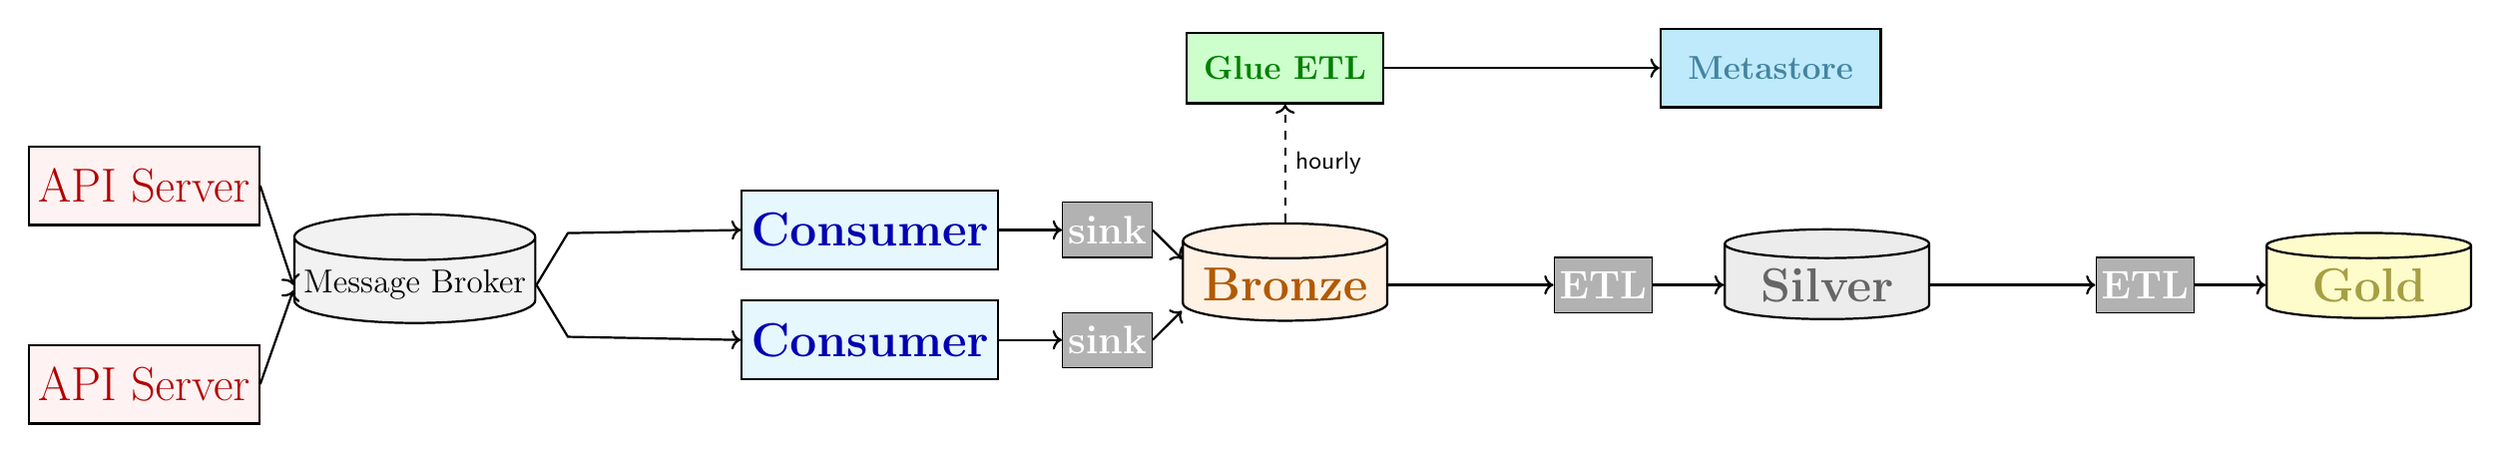
\begin{tikzpicture}[
        font=\sffamily,
        % 노드 스타일
        apiServer/.style={
            draw,
            rectangle,
            minimum width=2.8cm,
            minimum height=1.0cm,
            thick,
            fill=red!5!white,
            text=red!70!black,
            font=\LARGE,
        },
        broker/.style={
            draw,
            cylinder,
            shape border rotate=90,
            aspect=0.19,
            minimum width=2.6cm,
            minimum height=1.0cm,
            thick,
            fill=gray!10,
            font=\large
        },
        consumer/.style={
            draw,
            rectangle,
            minimum width=2.8cm,
            minimum height=1.0cm,
            thick,
            fill=cyan!10,
            font=\LARGE\bfseries,
            text=blue!70!black
        },
        graybox/.style={
            draw,
            fill=gray!60,
            minimum width=1.1cm,
            minimum height=0.7cm,
            text=white,
            font=\bfseries\Large,
            inner sep=2pt
        },
        bronze/.style={
            draw,
            cylinder,
            shape border rotate=90,
            aspect=0.19,
            minimum width=2.6cm,
            minimum height=1.0cm,
            thick,
            fill=orange!10,
            font=\LARGE\bfseries,
            text=orange!70!black
        },
        silver/.style={
            draw,
            cylinder,
            shape border rotate=90,
            aspect=0.19,
            minimum width=2.6cm,
            minimum height=1.0cm,
            thick,
            fill=gray!15,
            font=\LARGE\bfseries,
            text=gray!80!black
        },
        gold/.style={
            draw,
            cylinder,
            shape border rotate=90,
            aspect=0.19,
            minimum width=2.6cm,
            minimum height=1.0cm,
            thick,
            fill=yellow!20,
            font=\LARGE\bfseries,
            text=yellow!60!black
        },
        glueetl/.style={
            draw,
            rectangle,
            minimum width=2.5cm,
            minimum height=0.9cm,
            fill=green!20,
            thick,
            font=\large\bfseries,
            text=green!50!black
        },
        catalog/.style={
            draw,
            rectangle,
            minimum width=2.8cm,
            minimum height=1.0cm,
            fill=cyan!25,
            thick,
            font=\large\bfseries,
            text=cyan!60!black
        },
        myarrow/.style={thick,->}
    ]
    
    % 1. API Servers
    \node[apiServer] (API1) at (0,0.8) {API Server};
    \node[apiServer, below=1.5cm of API1] (API2) {API Server};
    
    % 2. Message Broker
    \node[broker, right=1.9cm of $(API1)!0.5!(API2)$] (MB) {Message Broker};
    
    % 3. Consumers
    \node[consumer, right=2.6cm of MB, yshift=0.7cm] (C1) {Consumer};
    \node[consumer, right=2.6cm of MB, yshift=-0.7cm] (C2) {Consumer};
    
    % 4. sink gray boxes  
    \node[graybox, right=0.8cm of C1] (sink1) {sink};
    \node[graybox, right=0.8cm of C2] (sink2) {sink};
    
    % 5. Bronze S3
    \node[bronze, right=0.95cm of $(sink1)!0.5!(sink2)$] (Bronze) {Bronze};
    
    % 6. ETL gray box
    \node[graybox, right=2.1cm of Bronze] (ETL1) {ETL};
    \node[silver, right=0.9cm of ETL1] (Silver) {Silver};
    \node[graybox, right=2.1cm of Silver] (ETL2) {ETL};
    \node[gold, right=0.9cm of ETL2] (Gold) {Gold};
    
    % 7. Glue ETL and Glue Catalog, placed above Bronze
    \node[glueetl, above=1.5cm of Bronze] (GlueETL) {Glue ETL};
    \node[catalog, right=3.5cm of GlueETL] (Catalog) {Metastore};
    
    % --- edges
    % API Servers to Broker
    \draw[myarrow] (API1.east) -- (MB.west);
    \draw[myarrow] (API2.east) -- ([yshift=-2pt]MB.west);
    
    % Broker to Consumers
    \draw[myarrow] (MB.east) -- ++(0.4,0.66) -- (C1.west);
    \draw[myarrow] (MB.east) -- ++(0.4,-0.66) -- (C2.west);
    
    % Consumers to sink box to Bronze
    \draw[myarrow] (C1.east) -- (sink1.west); 
    \draw[myarrow] (sink1.east) -- ($(Bronze.west)+(0,0.33)$);
    \draw[myarrow] (C2.east) -- (sink2.west); 
    \draw[myarrow] (sink2.east) -- ($(Bronze.west)+(0,-0.33)$);
    
    % Bronze -> ETL1 -> Silver -> ETL2 -> Gold
    \draw[myarrow] (Bronze.east) -- (ETL1.west);
    \draw[myarrow] (ETL1.east) -- (Silver.west);
    \draw[myarrow] (Silver.east) -- (ETL2.west);
    \draw[myarrow] (ETL2.east) -- (Gold.west);
    
    % Glue ETL -> Glue Catalog
    \draw[myarrow] (GlueETL.east) -- (Catalog.west);
    
    % Glue ETL -> Bronze (partition discovery)
    \draw[myarrow,dashed] (Bronze.north) -- (GlueETL.south) node[midway, right] {\small hourly};
    
    \end{tikzpicture}
    }

    \vspace{3mm}

    % ------------- 다이어그램 End
    
    \textbf{주요 성과}:
        
\begin{itemize}
    \item ETL 파이프라인 자동화 및 준실시간 탐색을 위한 크롤러 구축
\end{itemize}
\begin{itemize}
    \item Silver 티어를 파티셔닝, 버켓팅으로 저장하여 소규모 파일 문제를 해결하고, Silver 티어의 쿼리 속도를 \textbf{약 2.5배 향상}
\end{itemize}

    \resumeSubProjectListStart
        \resumeSubProject {\textbf{메달리온 아키텍쳐 설계}}
        {
        
        쿼리 사용자들, 다운스트림 ETL들의 조회 패턴을 분석하여, 그 결과를 토대로 파티셔닝과 버켓팅 전략을 설계하고 적용했습니다. 
        원시 데이터 보존을 통해 언제든 재처리가 가능하고, 각 단계별 데이터 검증(null 처리, 중복 처리, 데이터 타입 변환)을 통해 오류 데이터는 낮은 단계에 격리하여 상위 단계에서는 정확하고 고품질 데이터를 확보하였습니다. 
        이로써 분석과 비즈니스 활용에 최적화된 신뢰성 높은 데이터 환경을 구축하였습니다.
        % 원시 데이터(Raw, Bronze) → 정제 데이터(Clean, Silver) → 고품질 데이터(Gold)로 계층화하여
        % 오류나 결함이 있는 데이터는 낮은 단계에 가두고, 상위 단계에서는 깨끗한 데이터만 사용함으로써 품질 보장함.

        \vspace{1mm}
        \textbf{사용한 기술}: Amazon S3, Amazon Glue Data Catalog, Apache Spark
        \vspace{2mm}
        }
        \resumeSubProject {\textbf{데이터 수집 및 준실시간 파티션 등록}}
        
        {
        대용량 로그를 수집하기 위해 Kafka 기반의 스트리밍 플랫폼의 Consumer 그룹을 구축하고, Amazon Glue ETL로 준실시간 파티션 등록과 Spark 배치 처리를 병행하는 하이브리드 아키텍처를 설계했습니다.

        \vspace{1mm}
        \textbf{사용한 기술}: Apache Spark, Amazon Glue ETL, Kafka Connect
        \vspace{2mm}
    }
    \resumeSubProjectListEnd
  \resumeProjectListEnd

%-------------------------------------------
\section{\textbf{3. 침해곡 탐지 파이프라인 개편}}
  \resumeProjectListStart
    \resumeProject
    {\textbf{소속}: 드림어스컴퍼니} {}
    
    \textbf{기여도}: 임베딩 추출(Tensorflow) 제외하고 모두, 약 80\%
    
    {\textbf{설명}}:

        유통사에서 매일 신규 입수되는 7만$\sim$16만 곡의 오디오를 FLO 플랫폼 내 500만 곡의 보호 음원과 비교하여 침해곡을 판별하는 파이프라인을 구축/운영했습니다.

    \textbf{상황}:
    \begin{itemize}
        \item 유통사에서 매일 신규 입수되는 7만$\sim$16만 곡의 오디오를 FLO 플랫폼 내 500만 곡의 보호 음원과 비교하여 침해곡을 판별해야 하는 환경이었습니다.
        \item 유통사의 계약이 늘어나면서 최대 16만 곡을 처리하는 경우 최대 14시간으로 급증하였고, 실패시 하루를 넘어가는 문제가 발생했습니다.
        \item 불법 유통사의 새로운 어뷰징 기법 등장으로 인해 기존 방식의 탐지 정확도가 지속적으로 하락하는 문제가 발생했습니다.
    \end{itemize}
    
    \textbf{과제}: 
    \begin{enumerate}
        \item 대규모 음원 데이터 처리 성능을 개선하고 \textbf{침해곡 탐지 정확도 향상}
        \item 시스템 복잡도를 줄이면서 \textbf{소요 시간을 단축}하고 운영 비용을 절감할 수 있는 효율적인 파이프라인 재구축
    \end{enumerate}

    \vspace{3mm}

    \resizebox{0.95\textwidth}{!}{
        \begin{tikzpicture}[
            font=\sffamily,
            apiServer/.style={
                draw,
                rectangle,
                minimum width=2.9cm,
                minimum height=1.0cm,
                thick,
                fill=cyan!8,
                font=\large,
                align=center,
                text=black,
            },
            s3box/.style={
                draw,
                cylinder,
                shape border rotate=90,
                aspect=0.19,
                minimum width=2.1cm,
                minimum height=1.05cm,
                thick,
                fill=magenta!10,
                font=\Large,
                text=magenta!70!black,
                align=center,
            },
            vectordb/.style={
                draw,
                cylinder,
                shape border rotate=90,
                aspect=0.26,
                minimum width=2.4cm,
                minimum height=1.2cm,
                thick,
                fill=violet!10,
                font=\Large,
                text=violet!80!black,
                align=center,
            },
            notifbox/.style={
                draw,
                rectangle,
                thick,
                rounded corners=4pt,
                minimum width=2.9cm,
                minimum height=1.05cm,
                fill=green!13,
                font=\Large,
                text=green!40!black,
                align=center,
            },
            labelbox/.style={
                draw,
                rectangle,
                minimum width=0.95cm,
                minimum height=0.68cm,
                fill=gray!60,
                text=white,
                font=\bfseries,
                inner sep=2pt,
                align=center,
            },
            mysql/.style={
                draw,
                cylinder,
                shape border rotate=90,
                aspect=0.19,
                minimum width=2.1cm,
                minimum height=1.0cm,
                thick,
                fill=purple!20,
                font=\Large,
                text=purple!70!black,
                align=center,
            },
            cdn/.style={
                draw,
                rectangle,
                thick,
                minimum width=3cm,
                minimum height=1cm,
                fill=yellow!20,
                font=\large,
                align=center,
            },
            arr/.style={thick,->},
            dasharr/.style={thick,dashed,->,color=gray!70},
            node distance=0.4cm and 0.3cm
        ]
        
        % MySQL 노드 (추가)
        \node[mysql] (MySQL) at (0,0) {MySQL};
        
        % Preprocess 노드
        \node[apiServer, right=2.5cm of MySQL] (PP) {Preprocess};
        
        % 오디오 ID Read 라벨
        \node[labelbox, above=0.35cm of $(MySQL)!0.5!(PP)$] (readId) {read audioID};
        
        % S3 노드(첫번째)
        \node[s3box, right=2.3cm of PP] (S3A) {S3};
        
        % Embedding Extract 노드
        \node[apiServer, right=2.3cm of S3A] (EE) {Embedding\\Extract};
        
        % CDN 서버 노드 (서브 브랜치, 아래에)
        \node[cdn, below=1.5cm of EE] (CDN) {CDN};
        
        % Vector DB
        \node[vectordb, right=2.3cm of EE] (VDB) {Vector DB};
        
        % Filter
        \node[apiServer, right=2.3cm of VDB] (F) {Filter};
        
        % 두번째 S3 노드
        \node[s3box, right=2.3cm of F] (S3B) {S3};
        
        % Compile 노드
        \node[apiServer, right=2.3cm of S3B] (C) {Compile};
        
        % Slack Notify 노드
        \node[notifbox, right=2.3cm of C] (SN) {Slack};
        
        % 라벨링
        \node[labelbox, above=0.32cm of $(PP)!0.5!(S3A)$] (l1) {write};
        \node[labelbox, above=0.32cm of $(S3A)!0.5!(EE)$] (l2) {read};
        \node[labelbox, right=0.2cm of $(EE)!0.5!(CDN)$] (l3) {download audio files};
        \node[labelbox, above=0.32cm of $(EE)!0.5!(VDB)$] (l4) {write};
        \node[labelbox, above=0.32cm of $(VDB)!0.5!(F)$] (l5) {read};
        \node[labelbox, above=0.32cm of $(F)!0.5!(S3B)$] (l6) {write};
        \node[labelbox, above=0.32cm of $(S3B)!0.5!(C)$] (l7) {read};
    
        
        % 수평 화살표
        \draw[arr] (MySQL.east) -- (PP.west);
        \draw[arr] (PP.east) -- (S3A.west);
        \draw[arr] (S3A.east) -- (EE.west);
        \draw[arr] (EE.east) -- (VDB.west);
        \draw[arr] (VDB.east) -- (F.west);
        \draw[arr] (F.east) -- (S3B.west);
        \draw[arr] (S3B.east) -- (C.west);
        \draw[arr] (C.east) -- (SN.west);
        
        % CDN 분기 화살표 (Embedding Extract → CDN)
        \draw[arr] (EE.south) -- (CDN.north);
        
        % CDN → Embedding Extract (다운로드 후 리턴)
        % \draw[arr] (CDN.east) .. controls +(right:8mm) and +(down:6mm) .. (EE.south east);

        \end{tikzpicture}
    
    }
    \vspace{3mm}
    \textbf{주요 성과}:
    
    \begin{itemize}
        \item 대규모 500만 곡 데이터 환경에서 텍스트 유사도 연산과 임베딩 연산의 조합으로 동/변조곡 탐지 \textbf{정확도 18\%p 향상}(5\% $\rightarrow$ 23\%)
        \item Polars 기반 고성능 배치 처리와 Kubernetes 리소스 최적화로, \textbf{하루 운영 비용 73\% 절감}(\$12.4 $\rightarrow$ \$3.3, EC2 기준)
        \item 벡터 연산 및 데이터 처리 효율 극대화로, \textbf{총 소요 시간 53\% 단축}(최대 14시간 $\rightarrow$ 6.5시간)
    \end{itemize}
%     \begin{table}[ht]
% \centering

% \begin{tabularx}{\textwidth}{X c c}
% \toprule
% \textbf{성과 항목} & \textbf{절대 향상/절감} & \textbf{기존 $\rightarrow$ 개선} \\
% \midrule
% 대규모 500만 곡 환경에서 Polars 및 벡터 데이터베이스 적용으로 탐지 정확도 향상 & +18\,\%p & 5\,\% $\rightarrow$ 23\,\% \\
% Polars 기반 배치 처리 및 Kubernetes 리소스 최적화로 하루 운영 비용 절감 & –73\,\% & \$12.4 $\rightarrow$ \$3.3 \\
% 벡터 연산 및 데이터 처리 효율 극대화로 레포트 출력 시간 단축 & –53\,\% & 14\,h $\rightarrow$ 6.5\,h \\
% \bottomrule
% \end{tabularx}
% \end{table}

    
    \resumeSubProjectListStart
        \resumeSubProject {\textbf{정확도 향상을 위한 텍스트 유사도 연산 도입}}
        {
        
        도메인 특화 지식을 보유한 유관 부서와의 긴밀한 협업을 통해, 탐지 정확도를 높이는 핵심 솔루션으로 텍스트 유사도(레벤슈타인) 방식을 추가로 채택했습니다. 
        이에 따라 발생하는 대량의 텍스트 연산 부하를 해결하고 처리 속도를 극대화하기 위해, 메모리 효율성과 병렬 처리에 강점이 있는 Polars 엔진을 도입하여 시스템을 최적화했습니다.
        
        \vspace{1mm}
        \textbf{사용한 기술}: Python, Polars, asyncio
        \vspace{2mm}
        }
        \resumeSubProject {\textbf{임베딩 기반 유사도 연산 최적화를 위한 벡터 데이터베이스 도입}}
        {
        
        Python-native 코드로 수행하던 임베딩 기반 유사도(코사인 거리) 연산의 성능 한계를 느끼고, 
        획기적으로 단축시키기 위해 벡터 연산을 데이터베이스 계층에서 위임 처리하는 방안을 모색했고, 벡터 연산에 특화된 데이터 엔진인 PgVector를 도입하여 시스템을 최적화했습니다.
    
        \vspace{1mm}
        \textbf{사용한 기술}: Python, PgVector, Kubernetes(Amazon EKS), Amazon S3
        \vspace{2mm}
        }

        % \begin{itemize}
        %     \item Python 환경에서 대량의 텍스트 데이터를 처리할 때 발생하는 속도 저하 문제를 해결하기 위해, 메모리 효율성과 병렬 처리 성능이 우수한 데이터 엔진 도입을 고민했습니다.
        %     \item Python-native 코드로 수행하던 코사인 유사도 연산의 성능 한계를 느끼고, 획기적으로 단축시키기 위해 벡터 연산을 데이터베이스 계층에서 위임 처리하는 방안을 모색했습니다.
        % \end{itemize}
    \resumeSubProjectListEnd
  \resumeProjectListEnd

%-------------------------------------------
\section{\textbf{4. Trino 구축 및 운영}}
  \resumeProjectListStart
    \resumeProject
    {\textbf{소속}: 드림어스컴퍼니} {}
    
    \textbf{기여도}: Prometheus, Grafana 제외한 모든 작업
    
    {\textbf{설명}}:
    
    대규모 전사 멀티테넌트 데이터 플랫폼의 쿼리 엔진으로 사용되던 Amazon EMR 기반 Trino를 운영했습니다. 이 엔진은 고객의 이용권 정산 및 조회같은 중요한 배치 작업용 + 사내 데이터 조회용으로 사용되었습니다.
    
    
    \textbf{상황}: 
    \begin{itemize}
        \item Presto의 운영권이 기존 조직에서 저희 조직으로 이관되었고, Observability가 전혀 구축되어 있지 않아 성능 모니터링과 장애 대응이 어려운 상황이었습니다.
        \item 조직의 FinOps 정책으로 인해 불필요한 Worker EC2 비용 절감이 중요한 과제였습니다.
    \end{itemize}
    \textbf{과제}: 
    \begin{enumerate}
        \item 부족한 Observability를 구축하여 시스템 가시성 확보하고, 성능 모니터링과 장애 대응을 위한 모니터링 시스템 구축
        \item 사용자 쿼리 실패 시, 내결함성을 높이기 위한 자동 장애 대응
        \item 비개발자들과의 소통을 통해 헤비쿼리를 교정하고, 최적화
    \end{enumerate}

    %---------------- 주요 내용 End

    \vspace{6mm}

\begin{figure}[ht]
    \centering
   \resizebox{0.70\textwidth}{!}{
        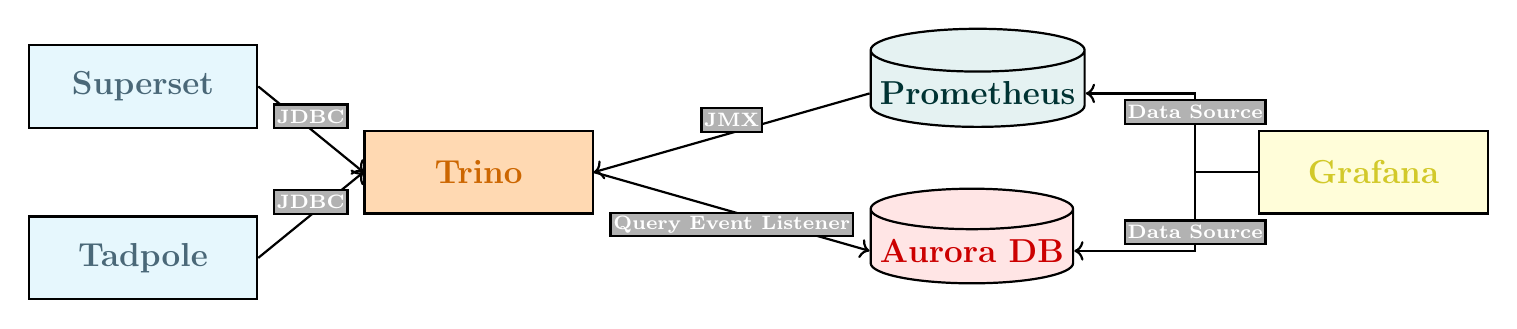
\begin{tikzpicture}[
    font=\sffamily,
    smallblock/.style={
        draw,
        rectangle,
        minimum width=2.9cm,
        minimum height=1.05cm,
        thick,
        fill=orange!30,
        font=\large\bfseries,
        align=center,
        text=orange!80!black
    },
    blueblock/.style={
        draw,
        rectangle,
        minimum width=2.9cm,
        minimum height=1.05cm,
        thick,
        fill=cyan!10,
        font=\large\bfseries,
        align=center,
        text=cyan!40!black
    },
    tealblock/.style={
        draw,
        cylinder,
        shape border rotate=90,
        aspect=0.20,
        minimum width=2.3cm,
        minimum height=1.05cm,
        thick,
        fill=teal!10,
        font=\large\bfseries,
        align=center,
        text=teal!40!black
    },
    redcylinder/.style={
        draw,
        cylinder,
        shape border rotate=90,
        aspect=0.20,
        minimum width=2.3cm,
        minimum height=1.05cm,
        thick,
        fill=red!10,
        font=\large\bfseries,
        align=center,
        text=red!80!black
    },
    beigeblock/.style={
        draw,
        rectangle,
        minimum width=2.9cm,
        minimum height=1.05cm,
        thick,
        fill=yellow!15,
        font=\large\bfseries,
        align=center,
        text=yellow!80!black
    },
    labelbox/.style={
        draw,
        rectangle,
        minimum width=0.6cm,
        minimum height=0.3cm,
        fill=gray!60,
        text=white,
        font=\scriptsize\bfseries,
        inner sep=1pt,
        align=center
    },
    arr/.style={thick,->},
    node distance=1.1cm and 1.5cm
]
% 노드들 위치 지정
\node[blueblock] (bi) at (0, 0.7) {Superset};
\node[blueblock, below=1.1cm of bi] (tadpole) {Tadpole};
\node[smallblock, right=2.8cm of $(bi)!0.5!(tadpole)$] (trino) {Trino};
\node[tealblock, right=3.5cm of trino, yshift=1.0cm] (prom) {Prometheus};
\node[redcylinder, right=3.5cm of trino, yshift=-1.0cm] (aurora) {Aurora DB};
\node[beigeblock, right=3.6cm of $(prom)!0.5!(aurora)$] (grafana) {Grafana};
% 화살표와 라벨 (수직/수평선만 사용)
\draw[arr] (bi.east) -- node[labelbox, above] {JDBC} (trino.west);
\draw[arr] (tadpole.east) -- node[labelbox, above] {JDBC} (trino.west);
\draw[arr] (prom.west) -- node[labelbox, above] {JMX} (trino.east);
\draw[arr] (trino.east) -- node[labelbox, below] {Query Event Listener} (aurora.west);
% Grafana -> Prometheus (ㄱ자 경로)
\draw[arr] (grafana.west) -- ++(-0.8,0) |- node[labelbox, above, pos=0.3] {Data Source} (prom.east);
% Grafana -> Aurora DB (ㄱ자 경로)  
\draw[arr] (grafana.west) -- ++(-0.8,0) |- node[labelbox, below, pos=0.3] {Data Source} (aurora.east);
\end{tikzpicture}        
        
    }
\end{figure}
    \vspace{3mm}
    
    \textbf{주요 성과}:
        \begin{itemize}
            \item Presto를 Trino로 전환하여 내결함성(Fault Tolerance)을 확보했고, 이를 통해 대규모 쿼리 처리 실패를 원천 차단하여 실패율 0\% 달성
            \item Observability 확보를 통해 쿼리 사용량 패턴을 분석하고, 사용량이 적은 시간대에 Worker 노드를 스케일 다운하는 \textbf{시간 기반 스케일링}을 도입하여 불필요한 Worker EC2 비용 \textbf{월 45\% 절감}
        \end{itemize}

    %---------------- 주요 성과 End

    \resumeSubProjectListStart
        \resumeSubProject {\textbf{Observability 강화를 위한 모니터링 구축}}
        {
        
        Trino 클러스터 운영의 효율성을 높이고 실시간 성능 모니터링과 장애 대응을 위해 Prometheus와 Grafana 기반의 통합 모니터링 시스템을 구축하였습니다. 이를 통해 쿼리 성능, 자원 사용 현황 등 다양한 메트릭을 시각화하고, 멀티테넌트 환경에서 발생할 수 있는 다양한 문제들에 대해 신속히 탐지 및 대응할 수 있는 체계를 마련하였습니다. 이 모니터링으로 인해 느린 쿼리를 발견하고 해결하였습니다.

        \vspace{1mm}
        \textbf{사용한 기술}: Prometheus, Grafana, MySQL, Python
        \vspace{2mm}
        }
    \resumeSubProjectListEnd

    %---------------- 서브 프로젝트 End

    \textbf{문제 해결(링크)}:
        \begin{itemize}
            \item \href{https://superhuman54.github.io/posts/trino-outofmemory/}{\textcolor{blue}{\underline{Trino 메모리 누수: Hadoop FileSystem Cache의 함정}}}
            \item \href{https://superhuman54.github.io/posts/trino-slow-query-analysis/}{\textcolor{blue}{\underline{Trino 느린 쿼리 분석과 성능 최적화}}}
        \end{itemize}
    
    %---------------- 트러블슛 End
    
  \resumeProjectListEnd

%-------------------------------------------
\section{\textbf{5. Amazon S3 기반 데이터레이크, 데이터웨어하우스 운영}}
  \resumeProjectListStart
    \resumeProject
    {\textbf{소속}: 드림어스컴퍼니} {}
    
    {\textbf{설명}:

    FLO 서비스에서 사용하는 RDBMS, MongoDB, 로그, 지표를 저장하는 데이터레이크와 데이터웨어하우스를 운영하고, 
    Spark, Amazon Glue Data Catalog로 필요한 데이터마트를 구성하였습니다. 
    또한, Airflow(Amazon MWAA)를 활용해 데이터 파이프라인 스케줄링 자동화를 구현하고, 
    클라이언트로 Kubernetes(Amazon EKS)를 사용하여 Amazon EMR과 상호작용하며 리소스 활용도와 운영 효율을 극대화하였습니다.

    \textbf{상황}:
    \begin{itemize}
        \item 시간 기반으로 스케줄링된 파이프라인들의 연쇄 작업 관리가 어려웠습니다.
        \item Groovy 스크립트로 작성된 Jenkins 파이프라인의 유지보수가 어려웠습니다.
        \item RDS를 데이터웨어하우스로 하루 한번 정기 배치로 적재하는 것으로는 DA의 긴급한 신규 테이블/컬럼 적재 요청에 대응하기 어려웠습니다.
    \end{itemize}

    \vspace{20mm}

    \begin{figure}[ht]
    \centering
   \resizebox{0.50\textwidth}{!}{
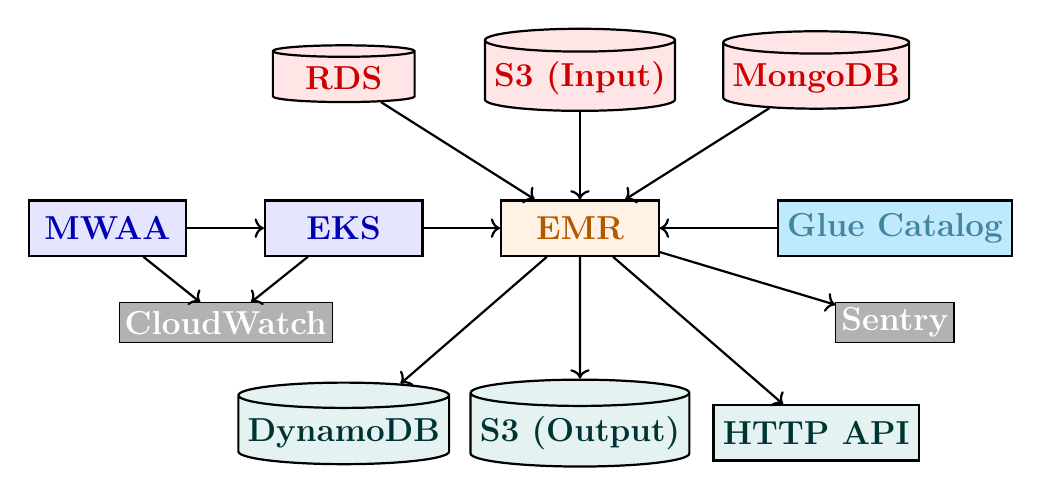
\begin{tikzpicture}[
    font=\sffamily,
    node distance=12mm,
% 노드 스타일
dist/.style={
    draw,
    rectangle,
    minimum width=2cm,
    minimum height=0.7cm,
    thick,
    fill=orange!10,
    font=\large\bfseries,
    text=orange!70!black,
},
orchestration/.style={
    draw,
    rectangle,
    minimum width=2cm,
    minimum height=0.7cm,
    thick,
    fill=blue!10,
    font=\large\bfseries,
    text=blue!70!black,
},
compute/.style={
    draw,
    rectangle,
    minimum width=2cm,
    minimum height=0.7cm,
    thick,
    fill=teal!10,
    font=\large\bfseries,
    text=teal!40!black,
},
catalog/.style={
    draw,
    rectangle,
    minimum width=2cm,
    minimum height=0.7cm,
    thick,
    fill=cyan!25,
    font=\large\bfseries,
    text=cyan!60!black,
},
inputstorage/.style={
    draw,
    cylinder,
    shape border rotate=90,
    aspect=0.12,
    minimum width=1.8cm,
    minimum height=0.5cm,
    thick,
    fill=red!10,
    font=\large\bfseries,
    text=red!80!black,
},
storage/.style={
    draw,
    cylinder,
    shape border rotate=90,
    aspect=0.12,
    minimum width=1.8cm,
    minimum height=0.5cm,
    thick,
    fill=teal!10,
    font=\large\bfseries,
    text=teal!40!black,
},
monitor/.style={
    draw,
    rectangle,
    minimum width=0.8cm,
    minimum height=0.5cm,
    fill=gray!60,
    font=\bfseries\large,
    text=white,
    inner sep=2pt,
},
myarrow/.style={thick,->},
]
% Orchestration
\node[orchestration] (mwaa)   at (0,  1.5)  {MWAA};
\node[orchestration] (eks)    at (3,  1.5)  {EKS};
\node[monitor]     (cw)       at (1.5, 0.3)   {CloudWatch};

\node[dist]     (emr)      at (6,  1.5)  {EMR};

\node[catalog]     (glue)     at (10,  1.5)  {Glue Catalog};
% --- input
\node[inputstorage]     (rds)      at (3,  3.4)    {RDS};
\node[inputstorage]     (mongodb)  at (6,  3.4)    {S3 (Input)};
\node[inputstorage]     (s3in)     at (9,  3.4)    {MongoDB};
% --- output
\node[storage]     (dynamodb) at (3, -1.1)  {DynamoDB};
\node[storage]     (s3out)    at (6, -1.1)    {S3 (Output)};
\node[compute]     (http)     at (9, -1.1) {HTTP API};

\node[monitor]     (sentry)   at (10,  0.3)   {Sentry};
% Edges
\draw[myarrow] (mwaa) -- (eks);
\draw[myarrow] (mwaa) -- (cw);
\draw[myarrow] (eks)  -- (cw);
\draw[myarrow] (eks)  -- (emr);
\draw[myarrow] (rds)     -- (emr);
\draw[myarrow] (glue)   -- (emr);
\draw[myarrow] (mongodb) -- (emr);
\draw[myarrow] (s3in)    -- (emr);
\draw[myarrow] (emr) -- (dynamodb);
\draw[myarrow] (emr) -- (s3out);
\draw[myarrow] (emr) -- (http);
\draw[myarrow] (emr) -- (sentry);
\end{tikzpicture}
}
\end{figure}

    \vspace{3mm}
    
    \textbf{주요 성과}:
        \begin{itemize}
            \item 워크플로우 스케줄러를 Jenkins에서 Airflow로 전환하여 언어, 플랫폼 일관성 확보로 개발 생산성 향상
            \item 새로운 컬럼, 테이블 등 데이터 모델링 요구사항을 확보하기 위해, ad-hoc 파이프라인을 구축하여 데이터 공급 체계 마련
        \end{itemize}
    
    }
    \resumeSubProjectListStart
    \resumeSubProject{\textbf{스케줄러 이관: Jenkins → Airflow, \textbf{기여도}: 30\%}}
    {
    
    DynamoDB, K8s Pod 등의 Airflow Operator 및 Sensor를 생성하고, DAG를 작성하여 모든 워크플로우를 모던 스케줄러로 이관하였습니다.
        \vspace{1mm}
        
        \textbf{사용한 기술}: Amazon MWAA, Python, Amazon EKS, Amazon Cloudwatch
        \vspace{2mm}
    }
    
    \resumeSubProject{\textbf{데이터 적재 자동화 \textbf{기여도}: 60\%}}
    {
    
    Amazon S3를 데이터 레이크로 구축하고 AWS Glue Catalog와 연동하여 메타데이터 관리를 체계화했습니다. 
    매일 수행되는 정기 배치 외에도, DA의 긴급한 신규 테이블/컬럼 적재 요청에 유연하게 대응하기 위해 Ad-hoc 파이프라인을 구축했습니다. 
    특정 테이블만 선별적으로 적재할 수 있는 Spark 애플리케이션을 개발하고, Airflow DAG Configuration으로 파라미터를 주입받아 실행하는 구조를 통해 신속한 데이터 공급 체계를 마련했습니다.

        \vspace{1mm}
        \textbf{사용한 기술}: Amazon Glue Catalog, Amazon MWAA, Spark
        \vspace{2mm}
    }

    \resumeSubProjectListEnd

    %---------------- 서브 프로젝트 End

    \textbf{문제 해결(링크)}:
        \begin{itemize}
            \item \href{https://superhuman54.github.io/posts/fail-to-releases-pods-on-the-same-k8s/}{\textcolor{blue}{\underline{공유 Kubernetes 클러스터에서 Airflow Pod 중복 생성 및 회수 실패 문제}}}
            \item \href{https://superhuman54.github.io/posts/conflict-between-emr-and-aws-sdk/}{\textcolor{blue}{\underline{Amazon EMR 6.12와 AWS Java SDK 충돌 문제}}}
            \item \href{https://superhuman54.github.io/posts/low-throughput-for-writing-to-dynamodb/}{\textcolor{blue}{\underline{Spark에서 DynamoDB 쓰기 성능 저하 문제}}}
            \item \href{https://superhuman54.github.io/posts/failed-to-release-completed-pod/}{\textcolor{blue}{\underline{Amazon MWAA에서 Kubernetes Pod 회수 실패 문제}}}
        \end{itemize}
    
    %---------------- 트러블슛 End

  \resumeProjectListEnd


%-------------------------------------------
\section{\textbf{6. PySpark에서 Polars로의 마이그레이션}}
  \resumeProjectListStart
    \resumeProject
    {\textbf{소속}: 드림어스컴퍼니} {}
    
    \textbf{기여도}: 100\%
    
    \textbf{상황}:
    \begin{itemize}
        \item 조직의 FinOps 정책으로 인해 불필요한 인프라 비용 절감이 중요한 과제였습니다.
        \item 소규모 EMR 클러스터가 프로비저닝 시간이 실제 집계 작업 시간보다 더 오래 걸리는 비효율적인 상황이었습니다.
    \end{itemize}
    
    \textbf{과제}:
    \begin{enumerate}
        \item 워크로드 특성 분석을 통해 분산 처리의 필요성을 재검토하고, 데이터 기반 의사결정을 통해 PySpark에서 Polars로 전환할 수 있는 근거를 확보하여 성능과 비용을 동시에 최적화
    \end{enumerate}
    
    \textbf{주요 성과}:
        \begin{itemize}
            \item 집계 작업 수행 시간 \textbf{85.42\% 감소} (4분 5초 → 36초)
            \item 하드웨어 스펙 축소: 8코어 48GB → 4코어 12GB
            \item 일일 운영 비용 \textbf{71.13\% 절감} (\$19.81 → \$5.72)
        \end{itemize}
    
    
    \resumeSubProjectListStart
    \resumeSubProject{\textbf{워크로드 특성 분석 및 단일 노드 엔진 전환}}
    {
    
    3개월간 워크플로우 지표 분석 결과 
    \begin{itemize}
        \item 데이터 볼륨이 일정(데이터셋이 단일 머신의 메모리 내에서 처리 가능한 중대 규모)
        \item 실제 작업 시간보다 클러스터 프로비저닝 시간이 더 오래 걸리는 워크플로우
    \end{itemize}
    를 고려하여 단일 노드 엔진으로 전환했습니다.
        \vspace{1mm}
        
        \textbf{사용한 기술}: Apache Spark, Polars, Amazon EKS
        \vspace{2mm}
    }

    \resumeSubProjectListEnd

    %---------------- 서브 프로젝트 End

    \textbf{문제 해결(링크)}:
        \begin{itemize}
            \item \href{https://superhuman54.github.io/posts/journey-to-polars/}{\textcolor{blue}{\underline{PySpark에서 Polars로의 마이그레이션: 85\% 성능 향상과 71\% 비용 절감}}}
        \end{itemize}
    
    %---------------- 트러블슛 End

  \resumeProjectListEnd


%-------------------------------------------
\section{\textbf{7. 추천 데이터 HTTP 서버 구축과 운영}}
  \resumeProjectListStart
    \resumeProject
    {\textbf{소속}: 드림어스컴퍼니} {}
    
    \textbf{기여도}: 100\%
    
    {\textbf{설명}:

    오프라인 추천 시스템 (정적 추천 시스템)을 운영하기 위한 사용자 추천 데이터를 조회하는 HTTP 서버를 운영했습니다.
    
    \textbf{상황}: 
    \begin{itemize}
        \item \textbf{API 문서를 수동으로 작성}하고 있어 생산성 저하와 API 작성자마다 다른 양식으로 인해 문서 관리가 어려웠습니다.
        \item 클라이언트는 MSA 아키텍처로 구성되어 있고, 각 서비스의 처리 시간이 곧 전체 응답 시간인데, \textbf{이 서버가 느리면 전체 응답 시간이 느려지는 문제}가 있었습니다.
        \item I/O 바운드 작업이 많았고, \textbf{모든 I/O 작업이 동기적으로 처리}되어 있었습니다.
    \end{itemize}
    
    \textbf{과제}: 
    \begin{enumerate}
        \item 클라이언트와의 원활한 협업을 위해 문서를 가급적 자동화하여 생산성 향상
        \item I/O 바운드 작업을 병렬 처리하여 응답 시간을 개선
        \item 사내 API의 공통적인 응답 템플릿이 있었지만, API 개발때마다 작성해야하는 번거로움 해결
    \end{enumerate}

    
    \textbf{주요 성과}:
    \begin{itemize}
        \item 기존 Flask 대비 비동기 처리 기반 FastAPI 도입으로 \textbf{API 요청 지연시간 76\%}(평균 500ms $\rightarrow$ 120ms) 감축 및 동시성 향상
        \item 타입 힌팅 적용과 Dependency Injection으로 코드 안정성과 유지보수성 강화
        \item FastAPI의 자동 문서 생성 기능으로 Swagger UI API 문서를 생성하여 생산성 향상
    \end{itemize}
    }

    \resumeSubProject{\textbf{FastAPI 전환 및 코드 품질 개선}}
    {
    
    기존 Flask 기반 HTTP 서버를 I/O 바운드 작업에 최적화된 FastAPI로 전환하면서, DynamoDB와 같은 외부 API 조회가 대량 발생하는 환경에서 응답 시간과 처리량이 향상되었습니다. FastAPI의 비동기 처리 덕분에 병목이 감소하며 전체 API 서버 성능이 크게 개선되었습니다. 또한, Dependency Injector를 활용해 코드 품질과 유지보수성 또한 강화했습니다.

    \vspace{1mm}
    \textbf{사용한 기술}: Python3.9, FastAPI, Dependency Injector, Amazon DynamoDB
    \vspace{2mm}
    }

    

  \resumeProjectListEnd

  
\end{document}